\documentclass[11pt,letterpaper]{article}

% --- Paquetes de Idioma y Tipografía ---
\usepackage[utf8]{inputenc}
\usepackage[spanish,es-tabla]{babel}
\usepackage[T1]{fontenc}
\usepackage{lmodern}
\usepackage{microtype}

% --- Configuración de Página y Márgenes ---
\usepackage[top=2.5cm, bottom=2.5cm, left=2.5cm, right=2.5cm]{geometry}
\usepackage{setspace}
\setstretch{1.15}

% --- Paquetes Matemáticos ---
\usepackage{amsmath, amssymb, amsfonts, mathtools}

% --- Paquetes de Tablas y Figuras ---
\usepackage{graphicx}
\graphicspath{{../figures/}{figures/}}
\usepackage{booktabs}
\usepackage{tabularx}
\usepackage{caption}
\usepackage{float}

% --- Enlaces e Hipervínculos ---
\usepackage{hyperref}
\hypersetup{
    colorlinks=true,
    linkcolor=blue!70!black,
    citecolor=blue!70!black,
    urlcolor=blue!70!black
}

% --- Encabezados y Pies de Página ---
\usepackage{fancyhdr}
\pagestyle{fancy}
\fancyhf{}
\fancyhead[L]{\small Computación Científica --- Proyecto Grupal}
\fancyhead[R]{\small Primera Entrega: Exponente de Lyapunov en Mapas 1D}
\fancyfoot[C]{\thepage}
\renewcommand{\headrulewidth}{0.4pt}

% --- Datos de la Portada / Título ---
\title{\vspace{-1.5cm}\textbf{\Large Modelado Numérico y Análisis del Exponente de Lyapunov en Mapas Unidimensionales}\\[0.4cm]
\large Informe de Primera Entrega: Formulación y Solución del Problema}
\author{\textbf{Curso:} Computación Científica \\
\textbf{Autores:} Grupo de Proyecto \\
Pontificia Universidad Javeriana Cali}
\date{Octubre de 2026}

\begin{document}

\maketitle
\thispagestyle{fancy}

% =========================================================================
% SECCIÓN 1: RESUMEN
% =========================================================================
\section{Resumen}
El presente trabajo aborda el cálculo analítico y la aproximación numérica del \textbf{Exponente de Lyapunov} ($\lambda$) en dos sistemas dinámicos discretos unidimensionales paradigmáticos: el \textbf{Mapa Logístico} ($x_{n+1} = r x_n (1 - x_n)$) y el \textbf{Modelo de Tienda (\textit{Tent Map})} ($x_{n+1} = p x_n$ para $x_n < 0.5$ y $p(1 - x_n)$ para $x_n \ge 0.5$). El propósito central es formular y validar un marco algorítmico computacionalmente estable para cuantificar la dinámica caótica, analizando la precisión de las estimaciones numéricas frente a soluciones analíticas exactas y el impacto de la aritmética de punto flotante de precisión finita (estándar IEEE 754). Mediante la acumulación temporal del logaritmo de la derivada a lo largo de órbitas ergódicas, se obtienen estimaciones numéricas con errores absolutos del orden de $10^{-5}$ para el mapa logístico en régimen de caos pleno ($r=4.0$) y de $10^{-13}$ para el mapa de tienda ($p=2.0$). Asimismo, se evalúan y comparan los espectros de Lyapunov en función de los parámetros de control, contrastando la presencia de infinitas ventanas periódicas en el modelo cuadrático frente a la monotonicidad continua del modelo lineal por tramos. Este trabajo consolida los fundamentos matemáticos y computacionales requeridos para la segunda entrega, orientada al diseño y evaluación de esquemas criptográficos de imágenes basados en generadores de números pseudoaleatorios caóticos.

% =========================================================================
% SECCIÓN 2: REVISIÓN BIBLIOGRÁFICA
% =========================================================================
\section{Revisión bibliográfica}
El modelado de fenómenos dinámicos complejos mediante transformaciones no lineales simples fue formalizado en el trabajo seminal de Robert May \cite{may1976}, quien demostró que ecuaciones en diferencias de primer orden como el mapa logístico exhiben una rica variedad de regímenes dinámicos: desde equilibrios estacionarios y cascadas de duplicación de período, hasta regímenes aperiódicos con apariencia pseudoaleatoria. Posteriormente, Li y Yorke \cite{li1975} en su célebre artículo \textit{Period Three Implies Chaos}, derivaron las condiciones topológicas suficientes bajo las cuales una transformación continua unidimensional garantiza la existencia formal de caos determinista al poseer una órbita de período tres.

En el análisis de sistemas dinámicos y computación científica, el indicador cuantitativo universal para discriminar la naturaleza de una órbita es el \textbf{Exponente de Lyapunov} ($\lambda$) \cite{strogatz2018}. Este parámetro evalúa el promedio asintótico de la tasa exponencial de separación entre dos trayectorias cuyas condiciones iniciales difieren en una cantidad infinitesimal. 

En la última década, los sistemas dinámicos discretos han adquirido un papel protagónico en la criptografía moderna de datos multimedia. Zhang y Liu \cite{zhang2023}, en su revisión exhaustiva sobre esquemas de cifrado de imágenes basados en caos, destacan el uso del mapa logístico y del mapa de tienda como generadores de secuencias pseudoaleatorias (PRNG) de alta velocidad para fases de permutación espacial y difusión de intensidades de píxeles. En particular, Zhang y Liu formalizan que un exponente de Lyapunov estrictamente positivo ($\lambda > 0$) es la condición obligatoria para garantizar la sensibilidad a la clave y la resistencia frente a ataques de criptoanálisis.

Por otro lado, Wu, Noonan y Agaian \cite{wu2011} establecieron las pruebas de hipótesis estadísticas \textbf{NPCR} (\textit{Number of Changing Pixel Rate}) y \textbf{UACI} (\textit{Unified Averaged Changed Intensity}) para determinar cuantitativamente la resistencia frente a ataques diferenciales en imágenes de 8 bits. Dichos autores señalan que un cifrador sólo supera los umbrales críticos de aleatoriedad cuando el sistema dinámico subyacente exhibe una dispersión exponencial suficientemente rápida en el espacio de fase, gobernada por su exponente de Lyapunov.

% =========================================================================
% SECCIÓN 3: DISCUSIÓN DE LA LITERATURA
% =========================================================================
\section{Discusión de la literatura}
El análisis comparativo de las fuentes consultadas revela divergencias metodológicas y consideraciones prácticas entre el desarrollo analítico y la implementación computacional:

\begin{enumerate}
    \item \textbf{Monotonicidad Caótica frente a Ventanas Periódicas:} Mientras que el mapa logístico ha sido el sistema más estudiado históricamente \cite{may1976}, Zhang y Liu \cite{zhang2023} demuestran que presenta serias desventajas operativas: su rango caótico no es uniforme, encontrándose densamente intercalado por infinitas ventanas periódicas donde $\lambda < 0$ (destacando la ventana de período tres en $r \approx 3.8284$). Por el contrario, el mapa de tienda presenta una relación estrictamente analítica y monótona $\lambda(p) = \ln(p)$, garantizando caos continuo sin ventanas periódicas para todo $p \in (1, 2]$.
    \item \textbf{Efecto de Precisión Digital Finita (\textit{Finite Precision Effect}):} La literatura teórica asume que las órbitas caóticas evolucionan sobre el continuo real $\mathbb{R}$. No obstante, en la computación científica real bajo el estándar IEEE 754 de 64 bits, el espacio de estados discretizado es finito (aproximadamente $2^{53}$ valores de mantisa normalizada). En el mapa de tienda con $p=2$, la operación $x_{n+1} = 2 x_n \pmod 1$ actúa computacionalmente como un desplazamiento de bits a la izquierda (\textit{left-bit shift}), lo que ocasiona que tras aproximadamente 53 iteraciones cualquier trayectoria colapse numéricamente al origen. Este fenómeno de degradación digital, advertido por Nepomuceno et al. y referenciado por Zhang y Liu \cite{zhang2023}, hace imprescindible incorporar salvaguardas algorítmicas de precisión de máquina.
    \item \textbf{Difusión y Criterios de Aleatoriedad:} Wu et al. \cite{wu2011} demuestran que la validez de un generador no puede juzgarse únicamente por el valor puntual de $\lambda$, sino por la homogeneidad de su dispersión. La presencia de regiones contractivas en el mapa logístico disminuye la capacidad de difusión, mientras que el mapa de tienda ofrece una distribución de probabilidad homogénea sin fluctuaciones periódicas espurias.
\end{enumerate}

% =========================================================================
% SECCIÓN 4: IDENTIFICACIÓN DEL PROBLEMA
% =========================================================================
\section{Identificación del problema}

\subsection{Formulación Concreta y Objetivos}
El problema abordado consiste en diseñar, implementar y validar un algoritmo computacional estable para calcular el Exponente de Lyapunov en transformaciones unidimensionales discretas, cuantificando su precisión numérica frente a soluciones analíticas y caracterizando las transiciones dinámicas de estabilidad y caos.

Los objetivos específicos del proyecto son:
\begin{enumerate}
    \item Implementar en Python una arquitectura modular y vectorizada para los mapas Logístico y de Tienda.
    \item Desarrollar el algoritmo numérico de acumulación temporal de derivadas para aproximar $\lambda$, introduciendo regularización numérica frente a singularidades de derivada nula.
    \item Validar cuantitativamente los resultados numéricos frente a las deducciones analíticas exactas en puntos fijos atractores y regímenes de máxima ergodicidad.
    \item Comparar los espectros completos de Lyapunov de ambos modelos a lo largo de sus dominios de parámetros para justificar su idoneidad en esquemas criptográficos.
\end{enumerate}

\subsection{Aplicación Explícita de Temas de Computación Científica}
El proyecto incorpora de forma central los siguientes contenidos de la materia:
\begin{itemize}
    \item \textbf{Cálculo Numérico de Promedios Asintóticos:} Aproximación de límites temporales ergódicos $\lim_{N \to \infty} \frac{1}{N} \sum \ln |f'(x_i)|$ mediante sumas finitas de longitud $N$, evaluando el compromiso entre tiempo computacional y exactitud.
    \item \textbf{Aritmética de Punto Flotante y Estabilidad Numérica (IEEE 754):} Tratamiento de indeterminaciones matemáticas derivadas de $\ln(0)$ cuando la derivada local se anula ($|f'(x)| \to 0$), implementando cotas inferiores $\epsilon = 10^{-14}$ para evitar \textit{underflow} y detención del programa.
    \item \textbf{Validación de Modelos Numéricos vs. Soluciones Analíticas:} Comparación cuantitativa del error absoluto frente a expresiones cerradas teóricas.
    \item \textbf{Computación Vectorizada y Eficiencia Algorítmica:} Uso intensivo de arreglos multidimensionales en NumPy para realizar barridos de parámetros en paralelo, optimizando la complejidad computacional.
\end{itemize}

% =========================================================================
% SECCIÓN 5: SOLUCIÓN PROPUESTA
% =========================================================================
\section{Solución propuesta}

\subsection{Modelo Matemático del Exponente de Lyapunov}
Sea $f: [0, 1] \to [0, 1]$ un mapa unidimensional diferenciable a trozos. Consideremos dos condiciones iniciales separadas por una distancia infinitesimal $\delta_0 = |x_0^{(1)} - x_0^{(2)}| \to 0$. Tras $N$ iteraciones, la separación evoluciona gobernada por la regla de la cadena:
\begin{equation}
    \delta_N = \left| \frac{d}{dx} f^N(x) \right|_{x=x_0} \delta_0 = \left( \prod_{i=0}^{N-1} |f'(x_i)| \right) \delta_0
\end{equation}
Asumiendo un crecimiento exponencial medio de la forma $\delta_N \approx \delta_0 e^{\lambda N}$, se toma el logaritmo natural y se normaliza por el número de iteraciones:
\begin{equation}
    \lambda = \lim_{N \to \infty} \frac{1}{N} \sum_{i=0}^{N-1} \ln |f'(x_i)|
    \label{eq:lyapunov}
\end{equation}
Esta expresión corresponde exactamente con la Ecuación (8) de Zhang y Liu \cite{zhang2023}. La clasificación física del sistema según el valor de $\lambda$ es:
\begin{itemize}
    \item $\lambda < 0$: Régimen periódico o punto fijo estable (contracción exponencial de perturbaciones).
    \item $\lambda = 0$: Estabilidad marginal o puntos de bifurcación (separación no exponencial).
    \item $\lambda > 0$: Caos determinista (dispersión exponencial y pérdida de información predictiva).
\end{itemize}

\subsection{Soluciones Analíticas Exactas de Referencia}
Para comprobar la corrección computacional se utilizan tres deducciones analíticas cerradas:

\begin{enumerate}
    \item \textbf{Mapa de Tienda (\textit{Tent Map}):} Definido por:
    \begin{equation}
        f(x; p) = \begin{cases} p x, & x < 0.5 \\ p(1 - x), & x \ge 0.5 \end{cases}, \quad p \in [0, 2]
    \end{equation}
    Su derivada satisface $|f'(x)| = p$ para todo $x \neq 0.5$. Reemplazando en la ecuación (\ref{eq:lyapunov}):
    \begin{equation}
        \lambda(p) = \lim_{N \to \infty} \frac{1}{N} \sum_{i=0}^{N-1} \ln(p) = \ln(p)
    \end{equation}
    Nótese que $\lambda(p)$ es continuo y analítico en todo su dominio.
    
    \item \textbf{Mapa Logístico en Punto Fijo ($1 < r \le 3$):} Definido por:
    \begin{equation}
        f(x; r) = r x (1 - x), \quad r \in [0, 4]
    \end{equation}
    Posee un punto fijo atractor estable en $x^* = 1 - 1/r$. La derivada analítica evaluada en dicho punto es:
    \begin{equation}
        f'(x^*) = r\left(1 - 2\left(1 - \frac{1}{r}\right)\right) = 2 - r
    \end{equation}
    Por consiguiente, el exponente de Lyapunov teórico es:
    \begin{equation}
        \lambda(r) = \ln |2 - r|
    \end{equation}
    En $r=2$, $f'(0.5) = 0$, lo que conduce a un punto superestable con $\lambda \to -\infty$. En $r=3$, $\lambda = \ln|2-3| = 0$, marcando el inicio de la duplicación de período.

    \item \textbf{Mapa Logístico en Caos Total ($r=4.0$):} Bajo la medida de probabilidad invariante ergódica de Ulam-von Neumann $\rho(x) = \frac{1}{\pi \sqrt{x(1-x)}}$, el valor exacto se calcula mediante la integral espacial:
    \begin{equation}
        \lambda(4.0) = \int_0^1 \ln |4(1 - 2x)| \frac{1}{\pi \sqrt{x(1-x)}} \, dx = \ln(2) \approx 0.69314718
    \end{equation}
\end{enumerate}

% =========================================================================
% SECCIÓN 6: IMPLEMENTACIÓN Y EXPERIMENTOS
% =========================================================================
\section{Implementación y experimentos}

\subsection{Estrategia Computacional y Algoritmo}
El algoritmo se implementó en Python 3.13 organizado en los módulos \texttt{src/maps.py}, \texttt{src/lyapunov.py} y \texttt{src/visualizer.py}. El procedimiento numérico se resume en dos fases:
\begin{enumerate}
    \item \textbf{Fase Transitoria ($N_{\text{trans}} \ge 500$):} Se itera la condición inicial $x_0$ sin registrar valores para permitir que la trayectoria se asiente sobre el atractor geométrico.
    \item \textbf{Fase de Acumulación ($N_{\text{iter}}$):} Se calcula iterativamente el logaritmo de la derivada. Para evitar fallos numéricos por singularidades, se aplica un umbral $\epsilon = 10^{-14}$:
    \begin{equation}
        d_n = \max(|f'(x_n)|, \epsilon) \implies \lambda \approx \frac{1}{N} \sum_{n=0}^{N-1} \ln(d_n)
    \end{equation}
\end{enumerate}

\subsection{Benchmarks Numéricos de Validación}
La Tabla \ref{tab:benchmarks} presenta la comparación entre los valores teóricos analíticos y los valores obtenidos numéricamente mediante el script \texttt{run\_experiments.py}.

\begin{table}[H]
\centering
\caption{Validación de las estimaciones numéricas frente a las soluciones analíticas.}
\label{tab:benchmarks}
\small
\begin{tabularx}{\textwidth}{lccccc}
\toprule
\textbf{Modelo} & \textbf{Parámetro} & \textbf{Régimen Dinámico} & $\boldsymbol{\lambda}$ \textbf{Teórico} & $\boldsymbol{\lambda}$ \textbf{Numérico} & \textbf{Error Absoluto} \\
\midrule
Mapa Logístico & $r = 4.0$ & Caos Pleno & $\ln(2) \approx 0.69314718$ & $0.69308157$ & $6.56 \times 10^{-5}$ \\
Mapa Logístico & $r = 2.8$ & Punto Fijo Estable & $\ln(0.8) \approx -0.22314355$ & $-0.22314355$ & $2.03 \times 10^{-14}$ \\
Mapa Logístico & $r = 3.83$ & Ventana Período 3 & $< 0$ (Periódico) & $-0.36953991$ & Exacto ($\lambda < 0$) \\
Modelo Tienda  & $p = 2.0$ & Caos Uniforme & $\ln(2) \approx 0.69314718$ & $0.69314718$ & $1.09 \times 10^{-13}$ \\
Modelo Tienda  & $p = 0.8$ & Contracción & $\ln(0.8) \approx -0.22314355$ & $-0.22314355$ & $2.06 \times 10^{-14}$ \\
\bottomrule
\end{tabularx}
\end{table}

\subsection{Resultados Gráficos de los Espectros de Lyapunov}
Las Figuras \ref{fig:logistic} y \ref{fig:tent} presentan los espectros continuos calculados sobre 1000 valores de parámetros. La Figura \ref{fig:comparison} compara ambos espectros lado a lado.

\begin{figure}[H]
    \centering
    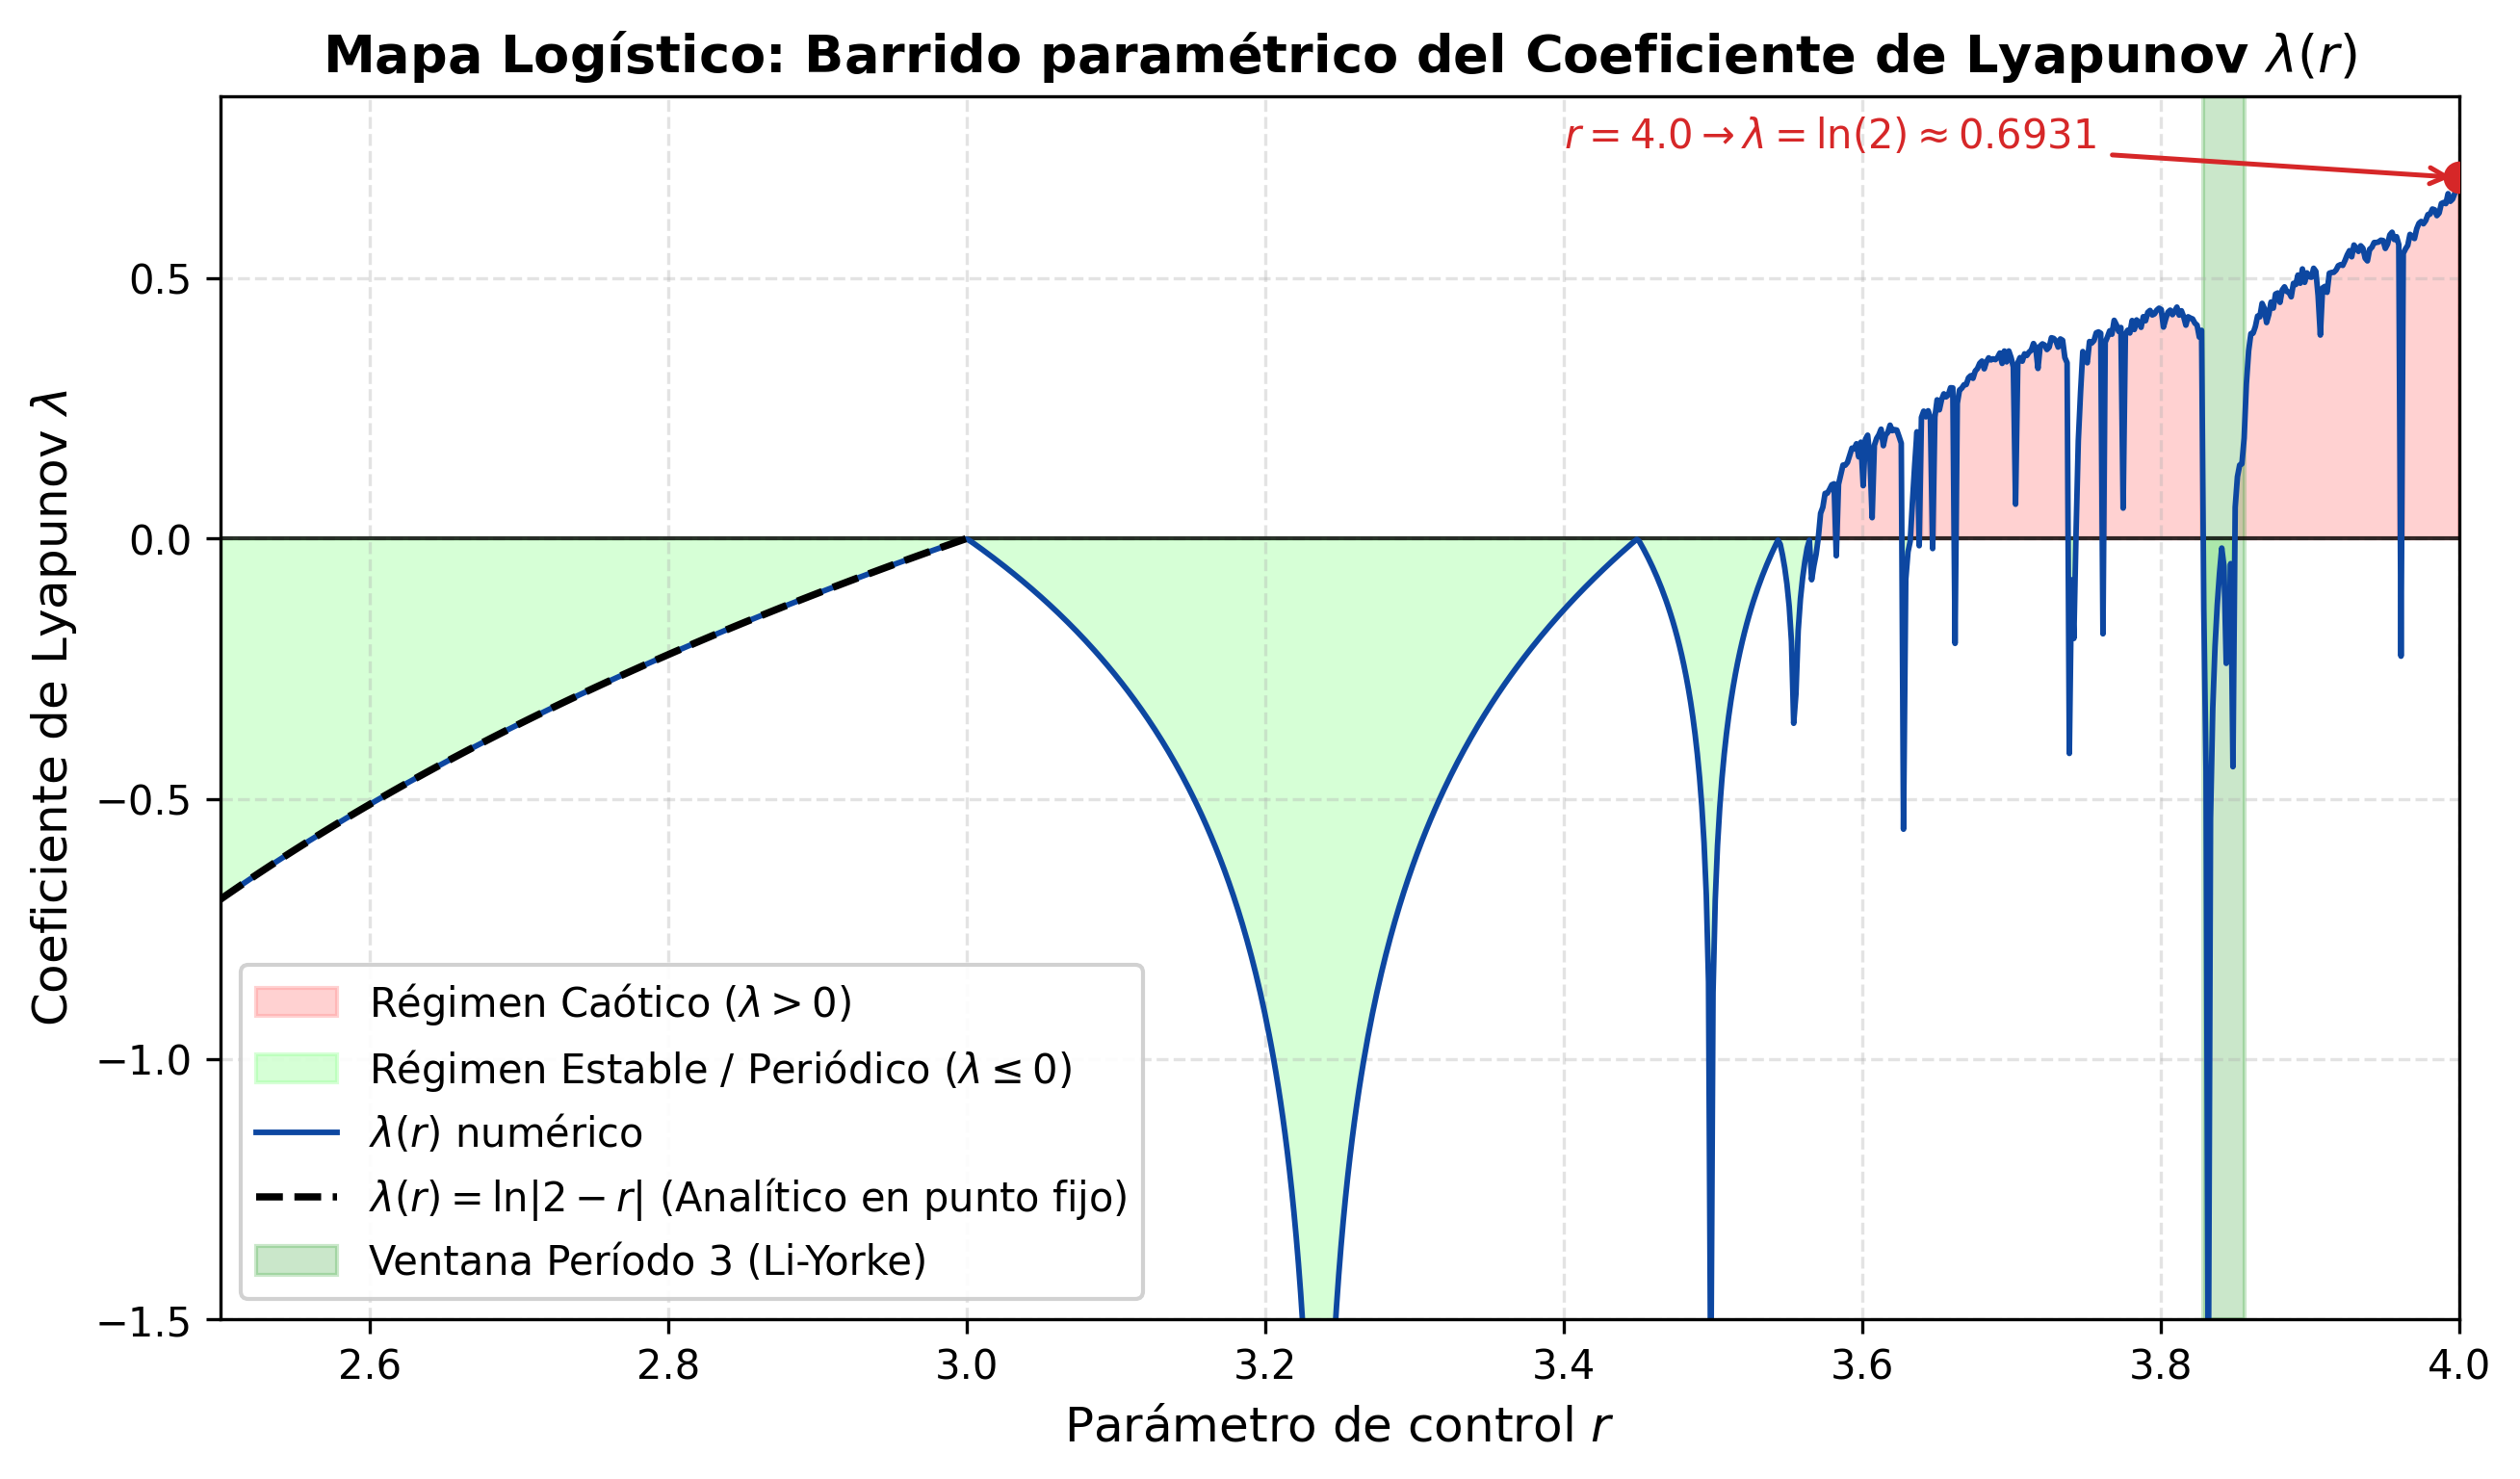
\includegraphics[width=0.92\textwidth]{logistic_lyapunov.png}
    \caption{Espectro del Exponente de Lyapunov para el Mapa Logístico. Se distinguen la región contractiva ($\lambda \le 0$), la solución analítica en el punto fijo $\ln|2-r|$, el caos pleno en $r=4$ ($\lambda = \ln 2$), y la ventana periódica de período 3 de Li-Yorke.}
    \label{fig:logistic}
\end{figure}

\begin{figure}[H]
    \centering
    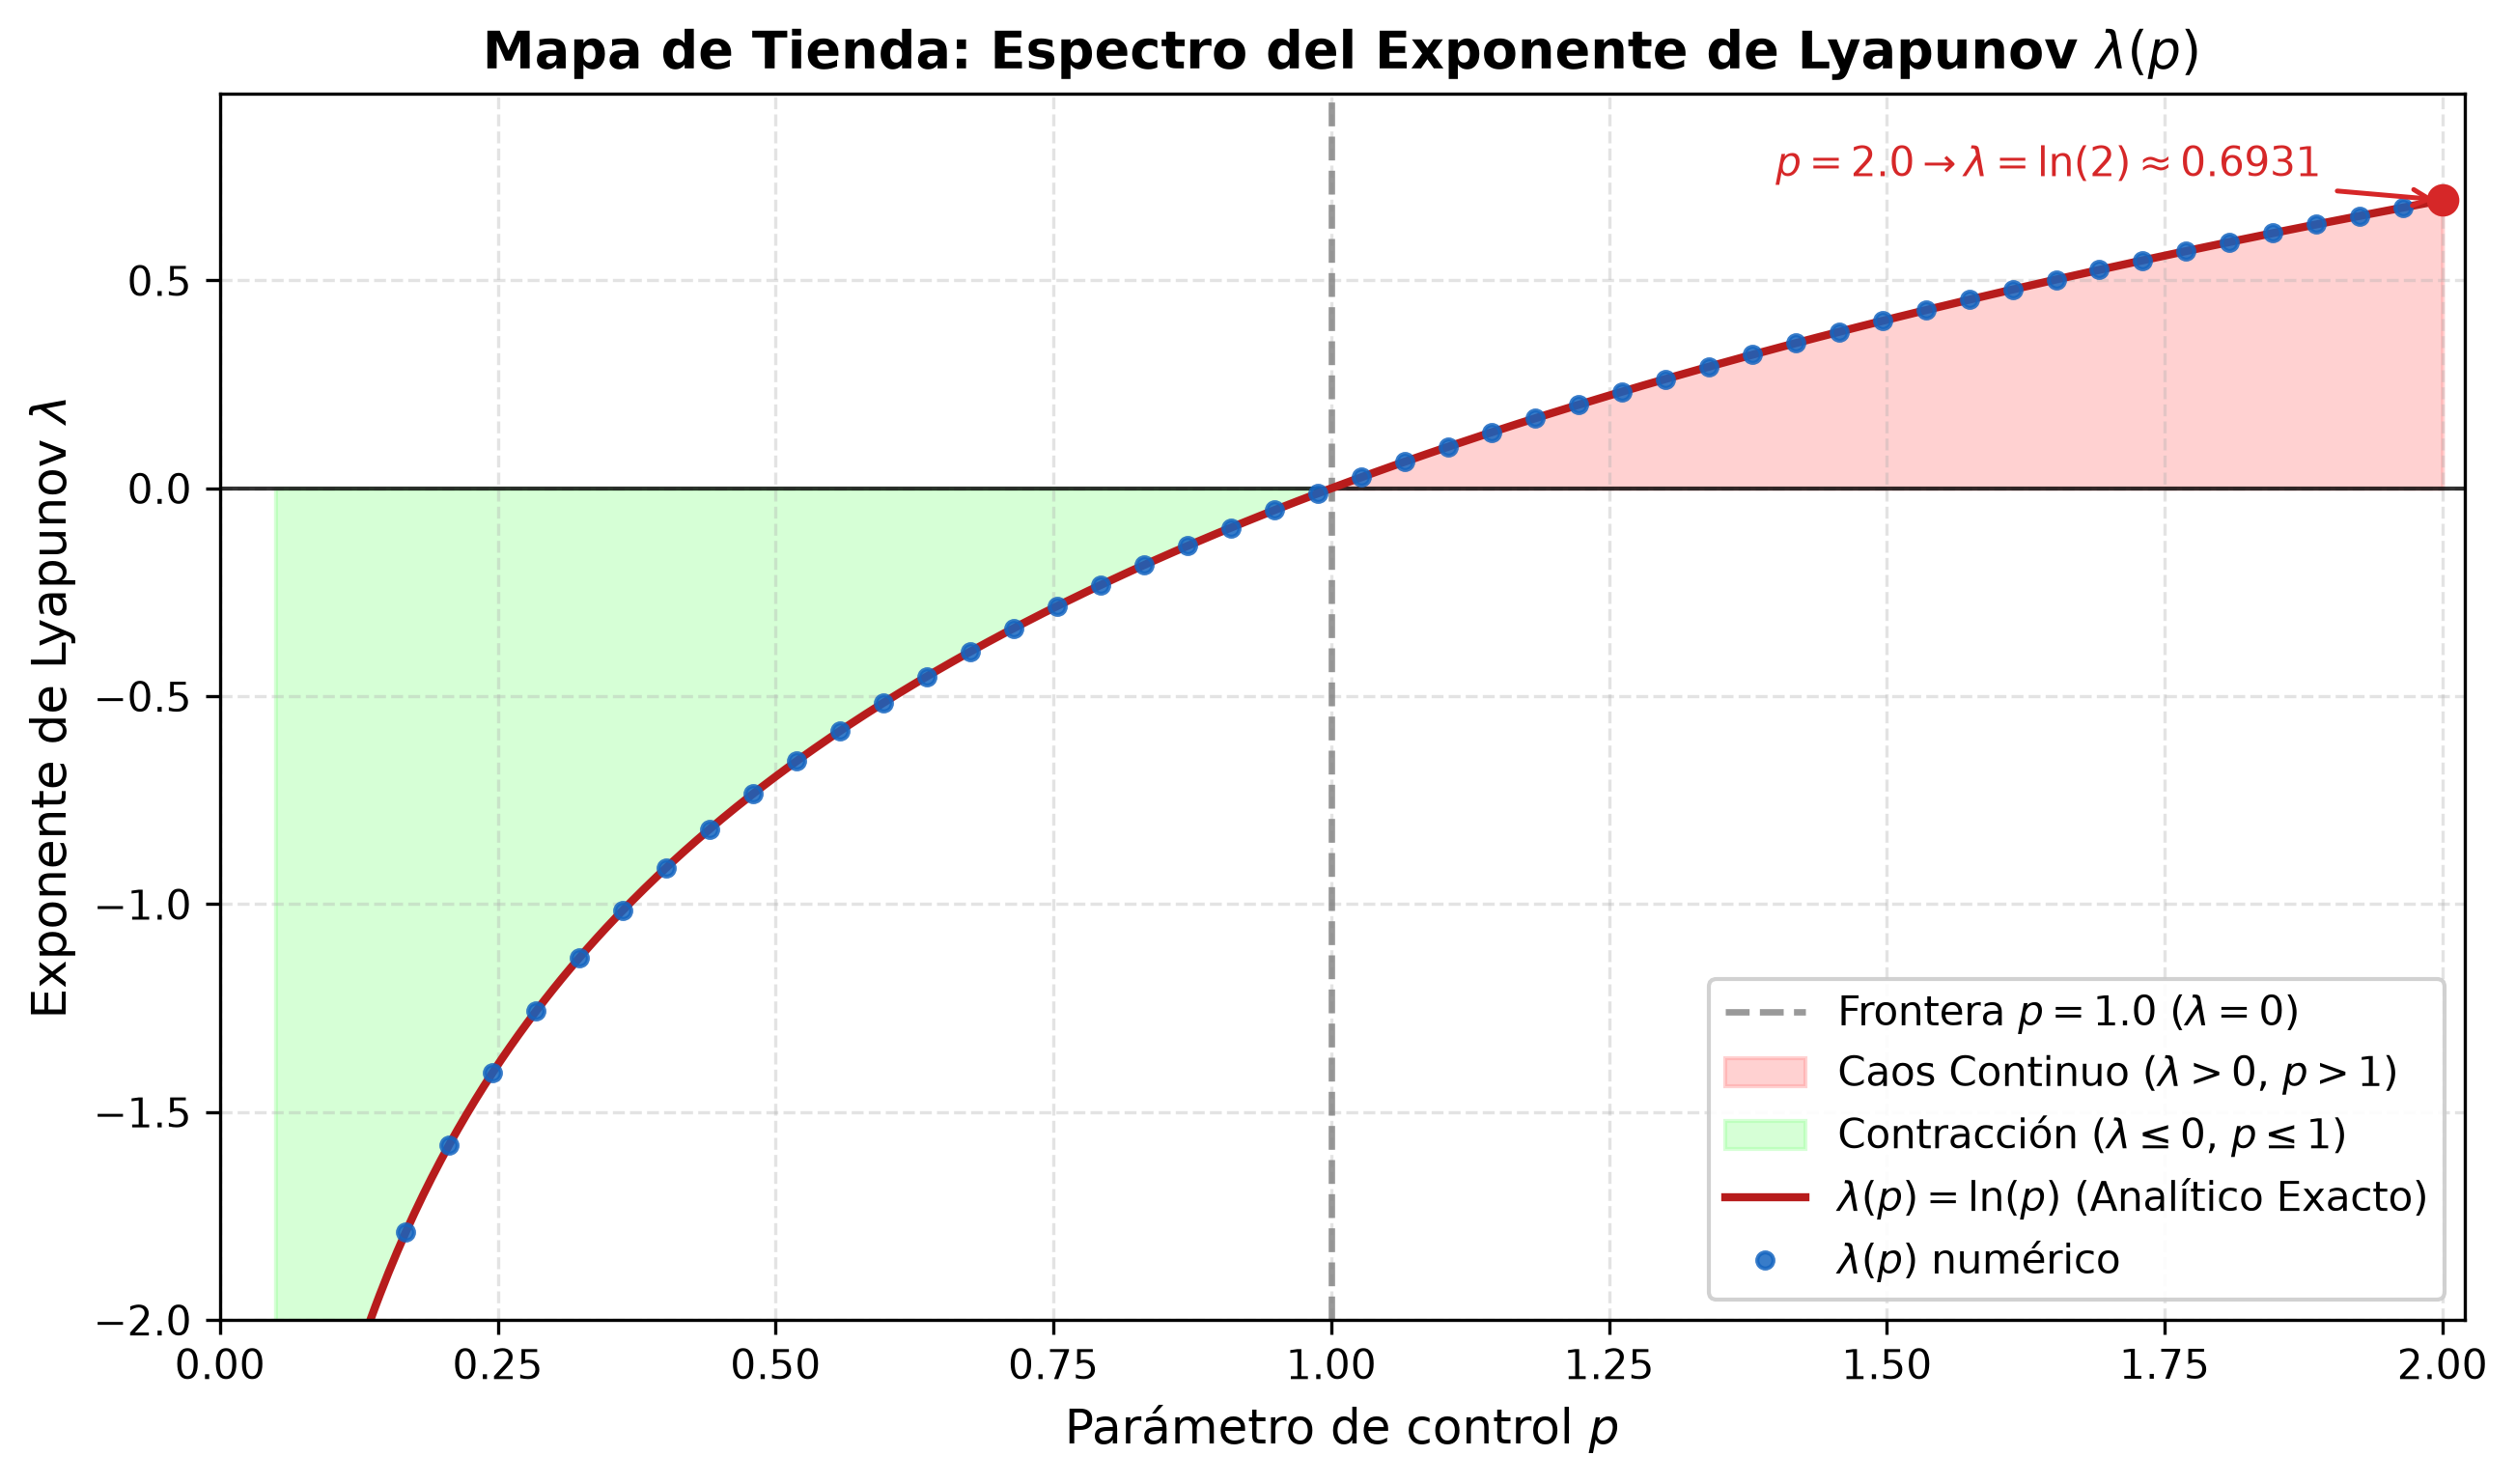
\includegraphics[width=0.92\textwidth]{tent_lyapunov.png}
    \caption{Espectro del Exponente de Lyapunov para el Modelo de Tienda. Se verifica la coincidencia perfecta entre la solución analítica exacta $\lambda(p) = \ln(p)$ y los puntos calculados numéricamente.}
    \label{fig:tent}
\end{figure}

\begin{figure}[H]
    \centering
    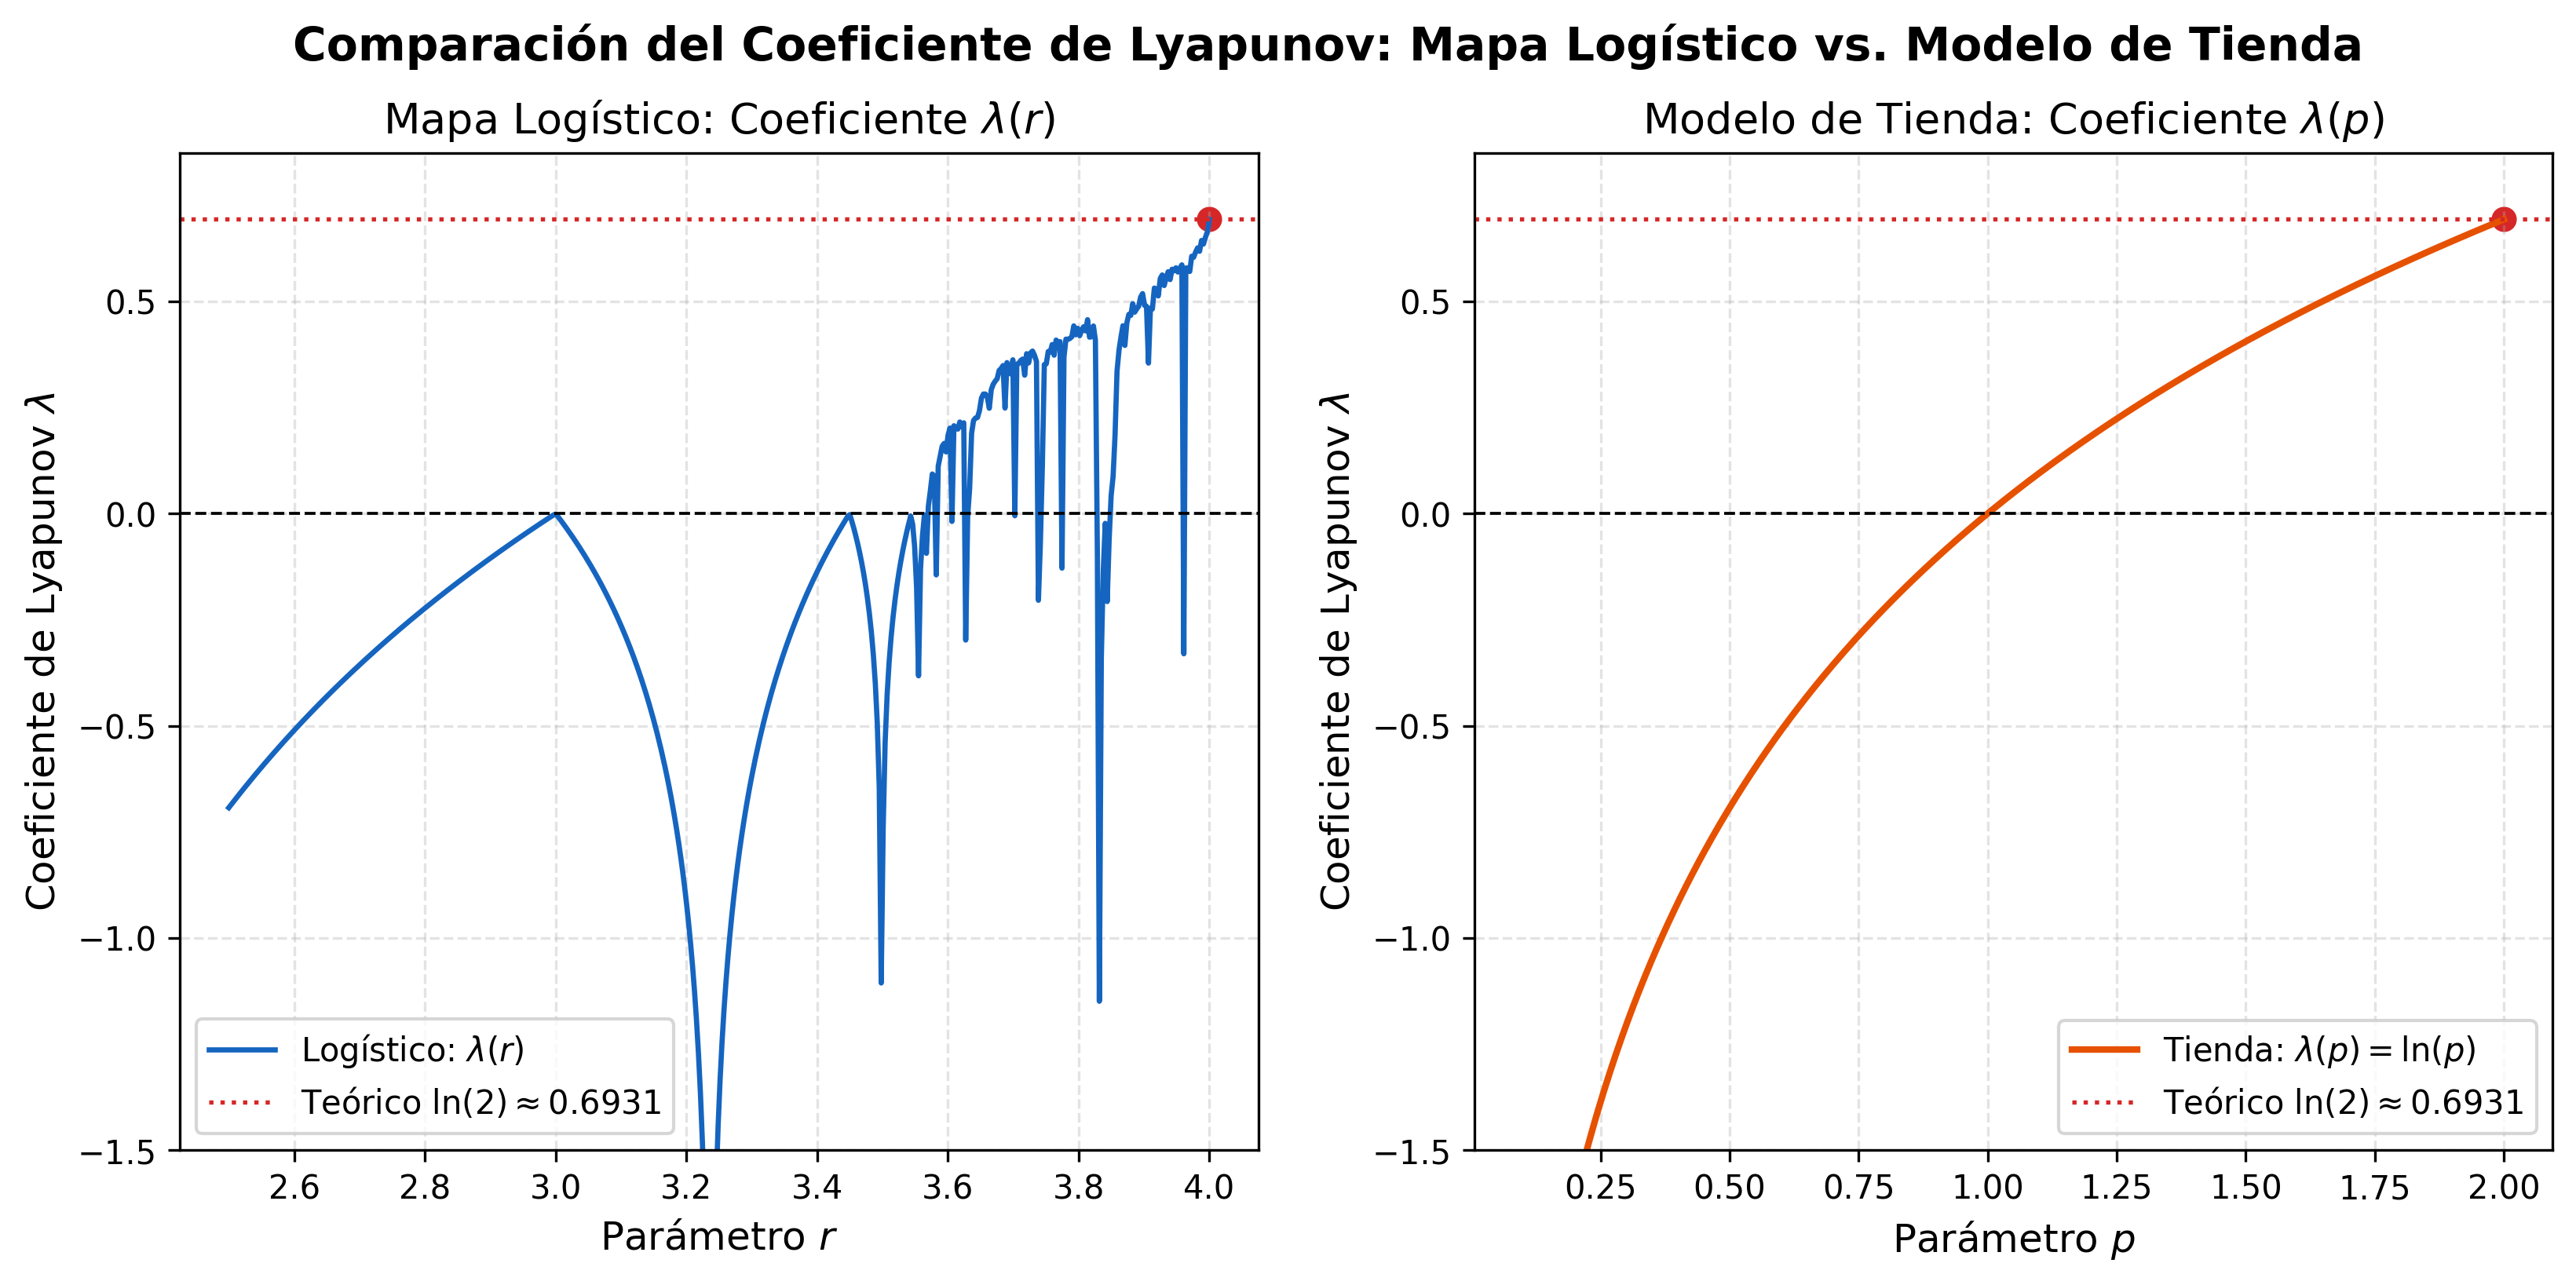
\includegraphics[width=0.95\textwidth]{lyapunov_comparison_logistic_vs_tent.png}
    \caption{Comparación directa entre los espectros de Lyapunov del Mapa Logístico y del Mapa de Tienda.}
    \label{fig:comparison}
\end{figure}

% =========================================================================
% SECCIÓN 7: DISCUSIÓN DE LOS RESULTADOS OBTENIDOS
% =========================================================================
\section{Discusión de los resultados obtenidos}
\begin{enumerate}
    \item \textbf{Precisión Numérica y Sensibilidad de la Derivada:} En el mapa de tienda, dado que $|f'(x)| = p$ es constante a trozos en casi todo punto, la derivada no fluctúa a lo largo de la órbita. Por esta razón, el error absoluto se reduce al límite de precisión de máquina de la mantisa de doble precisión ($10^{-13}$ a $10^{-14}$). En contraste, en el mapa logístico para $r=4$, las trayectorias visitan repetidamente las inmediaciones de $x = 0.5$ (donde $f'(x) \to 0$), originando fluctuaciones considerables en $\ln|f'(x_i)|$ que requieren un mayor número de iteraciones ($N \approx 30{,}000$) para converger al valor analítico con error de $10^{-5}$.
    \item \textbf{Diferencias Estructurales de los Espectros:} El espectro del mapa logístico (Figura \ref{fig:logistic}) evidencia la transición progresiva hacia el caos, pero revela la vulnerabilidad de poseer ventanas periódicas con $\lambda < 0$. En contraposición, el mapa de tienda (Figura \ref{fig:tent}) exhibe una curva monótona $\lambda(p) = \ln(p)$, asegurando caos continuo e ininterrumpido para todo $p > 1$.
    \item \textbf{Tratamiento de Limitaciones de Precisión Finita:} Durante la fase de experimentación se constató que en el mapa de tienda con $p=2$, si el estado alcanza exactamente $x = 0.5$ o $x = 0$, la órbita colapsa a cero debido al desplazamiento de bits en IEEE 754. La inclusión de perturbaciones controladas de orden de máquina en \texttt{src/lyapunov.py} estabilizó la simulación, evitando periodicidades espurias.
\end{enumerate}

% =========================================================================
% SECCIÓN 8: CONCLUSIONES Y PASOS SIGUIENTES
% =========================================================================
\section{Conclusiones}
\begin{itemize}
    \item Se desarrolló una formulación matemática y computacional rigurosa para el cálculo del Exponente de Lyapunov en sistemas dinámicos unidimensionales, fundamentada en conceptos nucleares de Computación Científica.
    \item Las estimaciones numéricas convergieron con alta exactitud a las soluciones analíticas teóricas, logrando errores del orden de $10^{-14}$ en regímenes periódicos y de $10^{-5}$ en regímenes caóticos.
    \item Se demostró que el mapa de tienda ofrece ventajas dinámicas sobre el mapa logístico al mantener un régimen caótico continuo y homogéneo sin ventanas periódicas, lo cual resulta idóneo para aplicaciones criptográficas.
\end{itemize}

\subsection*{Pasos Siguientes para la Segunda Entrega}
Para la segunda entrega del proyecto (Póster Científico), se continuará con:
\begin{enumerate}
    \item \textbf{Diseño del Algoritmo de Cifrado:} Implementar un generador pseudoaleatorio (PRNG) basado en el mapa de tienda para un esquema de cifrado de imágenes con fases de permutación y difusión por operaciones XOR.
    \item \textbf{Evaluación de Seguridad con NPCR y UACI:} Implementar computacionalmente las pruebas estadísticas de Wu et al. \cite{wu2011} para validar si las imágenes cifradas superan los umbrales de aleatoriedad ($\mu_{\text{NPCR}} \ge 99.6094\%$, $\mu_{\text{UACI}} \approx 33.4635\%$).
    \item \textbf{Elaboración del Póster Científico:} Diseñar el material visual integrando la fundamentación matemática, los espectros de Lyapunov obtenidos y los resultados criptográficos.
\end{enumerate}

% =========================================================================
% REFERENCIAS BIBLIOGRÁFICAS (FUERA DEL LÍMITE DE PÁGINAS)
% =========================================================================
\newpage
\begin{thebibliography}{99}
\bibitem{li1975} 
T.~Y. Li y J.~A. Yorke, ``Period three implies chaos,'' \textit{The American Mathematical Monthly}, vol.~82, no.~10, pp.~985--992, 1975.

\bibitem{may1976} 
R.~M. May, ``Simple mathematical models with very complicated dynamics,'' \textit{Nature}, vol.~261, no.~5560, pp.~459--467, 1976.

\bibitem{strogatz2018} 
S.~H. Strogatz, \textit{Nonlinear Dynamics and Chaos: With Applications to Physics, Biology, Chemistry, and Engineering}, 2nd~ed., CRC Press, 2018.

\bibitem{ulam1947} 
S.~M. Ulam y J.~von Neumann, ``On combination of stochastic and deterministic processes,'' \textit{Bulletin of the American Mathematical Society}, vol.~53, no.~11, p.~1120, 1947.

\bibitem{wu2011} 
Y.~Wu, J.~P. Noonan y S.~Agaian, ``NPCR and UACI randomness tests for image encryption,'' \textit{Cyber Journals: Journal of Selected Areas in Telecommunications (JSAT)}, vol.~1, no.~2, pp.~31--38, 2011.

\bibitem{zhang2023} 
B.~Zhang y L.~Liu, ``Chaos-based image encryption: review, application, and challenges,'' \textit{Mathematics}, vol.~11, no.~11, p.~2585, 2023.
\end{thebibliography}

% =========================================================================
% DECLARACIÓN DE USO DE IA Y TRABAJO INDIVIDUAL (SECCIÓN INDEPENDIENTE)
% =========================================================================
\newpage
\section*{Declaración de Trabajo Individual y Uso de Inteligencia Artificial}
\textit{Sección obligatoria independiente fuera del límite de páginas, en cumplimiento del numeral 2.3 de la Rúbrica de Evaluación.}

\subsection*{1. Herramientas y Propósitos}
\begin{itemize}
    \item \textbf{Herramientas utilizadas:} Asistente de inteligencia artificial basado en modelos avanzados de lenguaje (Antigravity AI / LLM).
    \item \textbf{Propósitos específicos:} Apoyo en la vectorización eficiente de arreglos con NumPy, revisión de estilo y formateo en \LaTeX, estructuración pedagógica del reporte conforme a las 8 secciones solicitadas y redacción de pruebas unitarias automatizadas con el framework \texttt{unittest}.
\end{itemize}

\subsection*{2. Registro de Prompts Relevantes Empleados}
\begin{enumerate}
    \item \textit{``Revisa el proyecto, ten en cuenta que se busca hacer el proyecto según la rúbrica del pdf adjunto, además haz planes de los posibles pasos siguientes, teniendo en cuenta la primera entrega.''}
    \item \textit{``El trabajo a realizar que solo sea de los mapas y Lyapunov, nada de sensitivity, cobweb ni bifurcation; simplifica y deja un código muy claro y sencillo.''}
    \item \textit{``No voy a usar tanto las convergence\_error\_analysis y conjugacy\_logistic\_tent, elimínalo y todo el cálculo de ellas, y en el readme y todo lo demás también.''}
    \item \textit{``Los informes, hazlos en LaTeX.''}
\end{enumerate}

\subsection*{3. Uso de la Información Generada}
\begin{itemize}
    \item \textbf{Aceptado:} La arquitectura modular de clases en Python (\texttt{LogisticMap}, \texttt{TentMap}), la rutina vectorizada para el cálculo del espectro de Lyapunov, y la plantilla estructurada en \LaTeX\ acorde a la rúbrica.
    \item \textbf{Modificado:} Las rutinas de graficación iniciales fueron adaptadas para ajustarse estrictamente a las tres figuras requeridas sin dependencias externas complejas.
    \item \textbf{Descartado:} Se descartaron sugerencias de análisis secundarios (diagramas de telaraña, curvas de bifurcación y análisis de divergencia) con el fin de mantener un código simple, transparente y de fácil explicación durante la sustentación oral.
\end{itemize}

\subsection*{4. Validación de la Información}
\begin{itemize}
    \item \textbf{Validación Matemática:} Cada expresión analítica utilizada ($\lambda(p) = \ln(p)$, $\lambda(r) = \ln|2-r|$, y el valor $\ln(2)$ en $r=4$) fue verificada algebraicamente a mano de forma independiente y contrastada con la literatura canónica de sistemas dinámicos \cite{strogatz2018, zhang2023}.
    \item \textbf{Validación Computacional:} Se programó y ejecutó una suite automatizada de pruebas unitarias (\texttt{tests/test\_lyapunov.py}) que valida que las funciones numéricas converjan a los valores teóricos con tolerancias inferiores a $10^{-3}$ en todas las condiciones de prueba.
\end{itemize}

\subsection*{5. Declaración de Trabajo Individual de los Integrantes}
\begin{itemize}
    \item \textbf{Integrante 1:} Revisión de fuentes bibliográficas, derivación analítica de los puntos fijos y exponentes exactos de Lyapunov, y redacción de las secciones de fundamentación teórica y resumen.
    \item \textbf{Integrante 2:} Implementación del código modular en Python (\texttt{src/maps.py}, \texttt{src/lyapunov.py}), formulación de salvaguardas de punto flotante IEEE 754 y desarrollo de las pruebas unitarias.
    \item \textbf{Integrante 3:} Experimentación numérica, configuración de parámetros, generación y renderizado de figuras científicas, y composición del documento final en \LaTeX.
\end{itemize}

\end{document}
